\chapter{Experiment Simulation}
\label{ch:Simulation}

Simulated data, or Monte Carlo (MC), plays a very important role in the \nova~analyses. The FD only expects $O(10^2)$ events per year, not nearly enough statistics to fine tune things like selection cuts. Furthermore, it is important that actual parameter measurements use an independent sample of data from that used to train and tune an anlysis. MC solves both of these problems by being explicitly different from the real data and having only computer memory limit statistics.

The full simulation chain is very long and comprises multiple steps, which reduces complexity and provides more opportunity for validation. At every step, the information from previous pieces of the simulation chain are kept so it is always possible to reproduce future results and trace any errors that may occur. The simulation chain consists of two main components, simulation of the beam and the detector response. This chapter discusses both of these areas in more detail, and finishes with a discussion of packages designed to study and validate the results.

\section{Flux Simulation}
\label{sec:SimFlux}

The first main simulation segment is the simulation of the NuMI beam, or the flux simulation. This section starts with the interaction of protons in the target and ends with experiment independent flux files full of neutrino rays that most importantly contain the flavor, direction, energy, and momentum of the neutrinos.

The flux simulation is performed using the FLUGG package, an interface between FLUKA \cite{ref:Fluka1, ref:Fluka2} and Geant4 \cite{ref:Geant41, ref:Geant42}. The version used for the analysis in this dissertation was FLUGG 2009.3, combining FLUKA2011 and Geant4 v4.9.6.p03(c). The FLUKA package is designed to simulate particle interactions and was used to simulate the proton interactions in the target. Geant4 is a toolkit for simulation of particles propagating through matter, and is used in this context to propagate the target interaction products through a detailed model of the NuMI beam line. This model of the beam includes all of the elements discussed in section \ref{sec:NuMI}, starting from the target hall all the way through the rock before the detector halls. The second focusing horn, a representative component of the geometry model, is shown in figure \ref{fig:GeomHorn}.
\begin{figure}[htb]
  \centering
  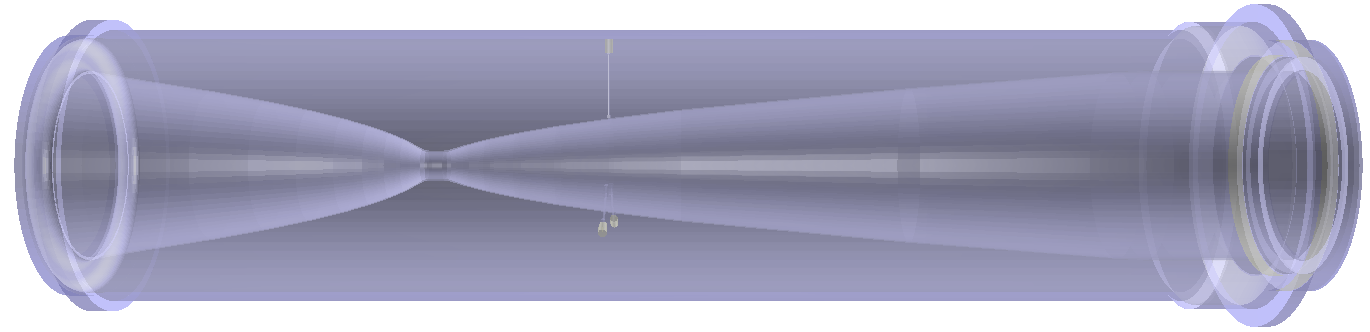
\includegraphics[width=0.9\textwidth]{figures/Horn2.png}
  \caption[Model of the Second Focusing Horn]{Visualization of the geometry used to model the second horn. This image was made during efforts to correctly position the three spider supports seen near the center of the schematic. Figure from \cite{ref:GeomNuMI}.}
  \label{fig:GeomHorn}
\end{figure}

The output of the FLUGG simulation is a set of flugg format flux files. These include the information described at the beginning of this section, but have several other key features as well. Simulating the particle products of every target interaction is extremely expensive on computing resources, so not every particle is tracked. Instead, similar neutrinos are often dropped in lieu of a single entry that is given a greater {\em importance weight}, one of two weights stored in the flux files. The information about the neutrino parent is also stored in the files, including the particle type, energy, momentum, and decay point. This affords later simulation steps the ability to ``re-decay'' a neutrino ray to a specific location and calculate the relative probability that this would occur. The latter value is stored as a {\em propagation weight}. Retaining the parent information also allows for event reweighting based on hadronic model studies.

The next piece of the flux simulation is largely a repackaging or the flugg format flux files into a unified format, called Dk2Nu \cite{ref:Dk2Nu}. FLUGG is certainly not the only flux generator, and \nova~is not the only experiment that uses the NuMI beam line. The Dk2Nu format is unified in the sense that it has the same format regardless of flux generator, and valid for any experiment using the NuMI beam.

Dk2Nu format flux files (or simply dk2nu files) are one of the main outputs from the flux simulation. However, one last step is taken to further simplify computation time for later simulation steps. The entries in the dk2nu files are sampled over a `window' that shadows the detector of interest, resulting only in a set of neutrino rays that could create interactions within the detector. The output files from this final step are in the GSimpleNtpFlux format, or more simply referred to as gsimple files \cite{ref:gsimple}.

\section{Detector Simulation}
\label{sec:SimDet}

The second main section in the simulation chain is the detector simulation. This section begins with neutrino interactions, models many different detector response effects, and finishes with files of simulated raw hits, or the signals read out by the detector electronics. The latter portion of this section closely follows the \nova~Simulation Technical Notes \cite{ref:TNDetSimFA, ref:TNDetSimSA}, which provide more detail and further references.

\subsection{Neutrino Interactions}
\label{sec:SimGENIE}

Neutrino interactions are modeled using the GENIE event generator product \cite{ref:GENIEGen, ref:GENIE}. For the analysis in this dissertation, version v2.10.4 was used. GENIE requires as input flux files, a model of the detector geometry, and cross section information, and from this determines if and where a neutrino interaction occurs, the type of interaction, and the kinematics of the interaction products. The generator uses a sophisticated model of the nucleus that allows for quasi-elastic, resonant, or deep inelastic scattering, taking into account any intranuclear scattering that may occur after the initial interaction takes place. The output of a GENIE interaction is a list of primary particles that escape the target nucleus and the relevant kinematic variables that describe each entry.

There is growing evidence \cite{ref:MinervaMEC, ref:NOvAFANuMu} that there is a type of nuclear interaction involving a quasi-bound nucleon-nucleon pair. This interaction is coined the meson exchange current, or MEC, and is included as an empirical model in GENIE. These events largely occur in an energy region between quasi-elastic (QE) and resonant (RES) events, vanishing by $5\unit{GeV}$ where QE scattering from free nucleons well model external data. While the inclusion of MEC interactions does not bring the data and MC into complete agreement, it substantially improves the discrepancy; see figure \ref{fig:MEC}. Consequently, an additional systematic error is evaluated for the MEC scale, discussed in chapter \ref{ch:Systs}. Furthermore, data used to constrain the empirical model in GENIE was only available for CC interactions, so there are no NC MEC events in the MC \cite{ref:TNGENIE}.
\begin{figure}[!p]
  \centering
  \begin{tabular}{c}
    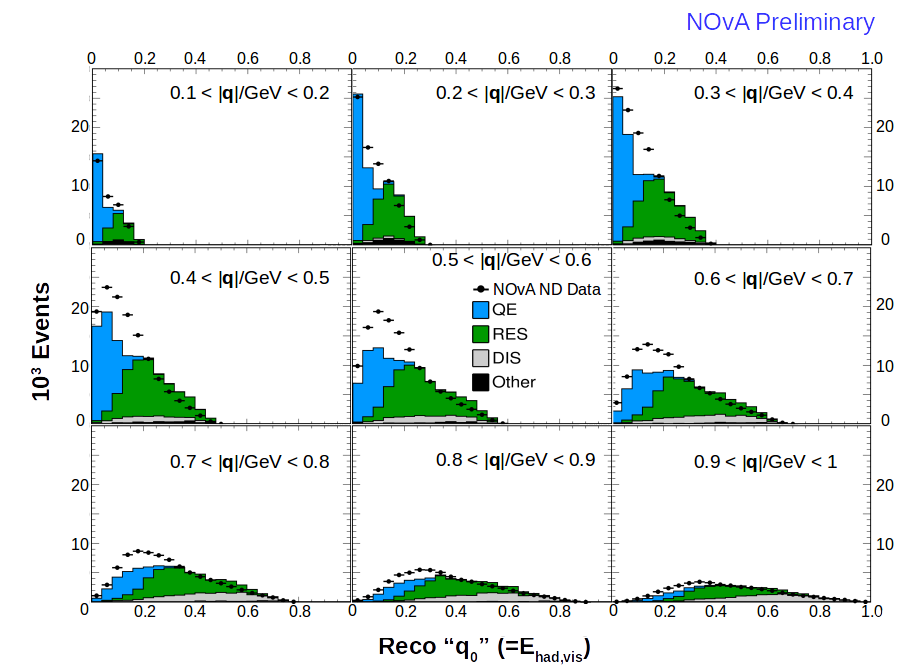
\includegraphics[width=.75\textwidth]{figures/MECOff.png} \\
    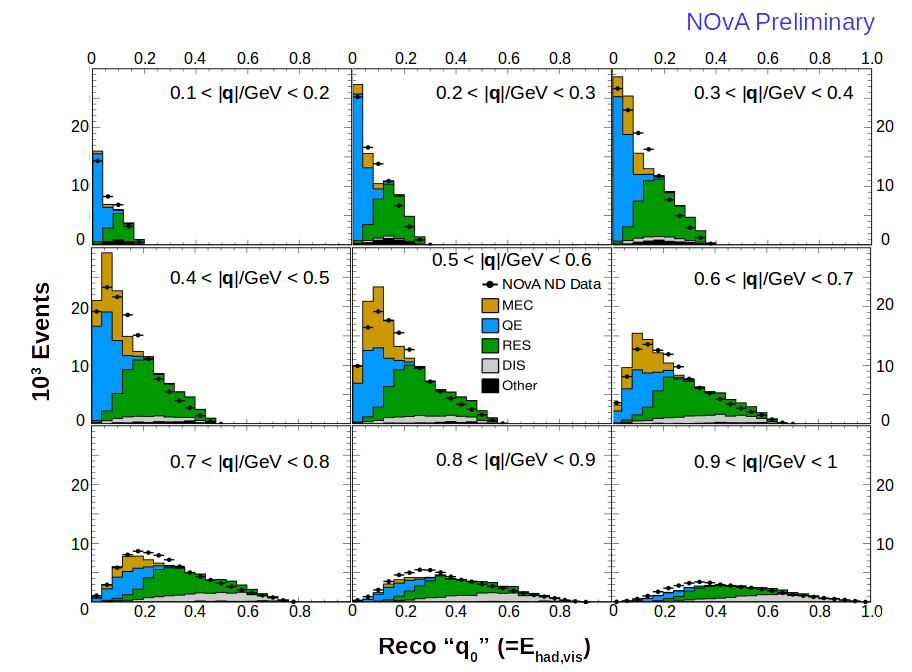
\includegraphics[width=.75\textwidth]{figures/MECOn.png} \\
  \end{tabular}
  \caption[Data/MC Comparison With and Without MEC Events]{Distributions of the reconstructed visible hadronic energy for different `slices' of estimated three momentum transfer, with (right) and without (left) MEC events. The events used for these distributions come entirely from ND selected $\numu$ CC events. Plots from \cite{ref:MECPlots}.}
  \label{fig:MEC}
\end{figure}

In truth, the actual `tuned' MEC model is applied as a weight on an event level, and there are a couple other effects applied in a similar fashion. The effect of long-range nuclear charge screening, or RPA (random phase approximation) suppression was studied by creating a shifted spectrum using a set of event weights. This shifted spectrum was translated into a systematic error band, assessed in chapter \ref{ch:Systs}. The single non-resonant pion production rate was decreased also using event weights to a level consistent with the most recent data studies \cite{ref:TNGENIE}.

The GENIE output is next fed back to Geant4 for particle propagation through the detector geometry \cite{ref:Geant41, ref:Geant42}. It models the primary particle interactions within the detector, including energy deposition and secondary interactions. The physical processes considered and modeled are somewhat configurable via the choice of the physics list. At this point in the simulation, it is much more important to accurately track the detailed interactions, so particles are not dropped as in the flux simulation; instead, a more precise model was used here. The specific physics list used was QGSP\_BERT\_HP, where QGSP specifies that high energy hadrons ($> 10\unit{GeV}$) are modeled with the quark gluon string model, BERT speficies that lower energy hadrons ($< 10\unit{GeV}$) are modeled with the Bertini cascade model, and HP toggles the usage of a high precision neutron model that tracks low energy neutrons ($< 20\unit{MeV}$) \cite{ref:TNDetSimFA}. The output from Geant4 at this stage is a list particles involved in the detector interaction and a full suite of information about each one, called the MC truth. The information that is most important to the next simulation step is a list of energy depositions and positions.

It is worth noting that the simulated events for the Near and far Detectors are generated somewhat differently. The FD expects a very low event rate per beam spill, while the ND expects multiple events per spill. As a result, the FD events are generated one at a time with the simulation calculating the POT needed for the event occur, and ND events are generated assuming a constant POT/spill and a variable number of events. Furthermore, the high rate of interactions at the ND means that it observes many muons that originate from neutrino interactions that begin in the rock outside of the detector. Most of these so called rock events do not result in any detector activity, so tracking them wastes valuable computing time. To deal with this, the ND detector events and single rock events are generated separately, and only the rock events that cause detector activity are kept. The final ND event records are made by overlaying rock events on the detector events. The number of rock singles to overlay is drawn from a Poisson distribution with a mean determined from data \cite{ref:SimRock}. A top down view of the neutrino interaction vertices at the ND is shown in figure \ref{fig:MCCO_NDVtx} and shows the level of detail used to model the geometry of the ND hall.
\begin{figure}[htb]
  \centering
  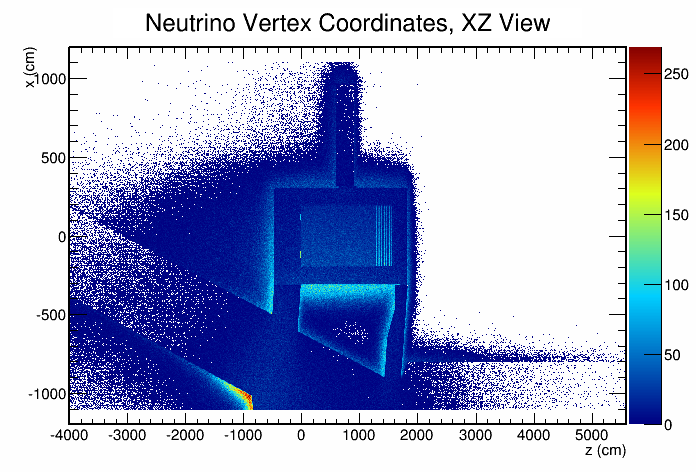
\includegraphics[width=0.75\textwidth]{figures/MCCO_NDXZ.png}
  \caption[ND Neutrino Interaction Vertex Distribution]{Distribution of neutrino interaction vertices in the XZ view at the ND hall. Several features of the geometry model can be seen. The detector sits between $\pm200\unit{cm}$ in X and $0 < \mbox{Z} < 1600\unit{cm}$. The muon catcher steel planes are easily identified at the back of the detector as the line segments with slightly enhanced interaction rates. The two small blips of greater activity at $\pm100\unit{cm}$ in X and $0\unit{cm}$ in Z are the bookend keeping the detector in place. The wide, sloped region extending from $0$ on the Z axis to $0$ on the X axis is an excavated pathway.}
  \label{fig:MCCO_NDVtx}
\end{figure}

Geant4 also handles the next piece of the simulation, the conversion between energy deposition and light yield. For low energies, the rate of light produced in liquid scintillator is proportional to the energy deposition, but the light yield begins to quench for particles with high enough energies. The Birks-Chou Law, encapsulated within a Geant4 module, is used to model the relationship between scintillator light yield rate, $\frac{dL}{dx}$, and particle energy deposition rate, $\frac{dE}{dx}$ \cite{ref:BirksChou}.

\beq
\frac{dL}{dx} = L_0 \frac{ \frac{dE}{dx} }{1 + k_B \frac{dE}{dx} + k_C \left( \frac{dE}{dx} \right)^2} 
\label{eq:BirksChou}
\eeq

\n Above, the constants $L_0$, $k_B$, and $k_C$ are dependent on the scintillator material and had to be estimated for \nova~as no measurement existed for the particular materials used in the experiment. A study was performed comparing the energy deposition at the end of proton tracks in the ND for both data and MC to find parameters that would generate agreement between the two \cite{ref:DanBirks}. The results of the study were $k_B = 0.04\unit{cm/MeV}$ and $k_C = -0.0005\unit{(cm/MeV)}^2$. The output from this simulation step is a set of energy depositions now encoded as light yield called FLSHits, or fiber in liquid scintillator hits.

\subsection{Photon Propagation}
\label{sec:Photon}

The next part of the simulation simulates the capture of the scintillation photons, their transport through the WLS fiber to the electronics, and their conversion into photoelectrons after collection by the APD. The detector is treated as uniform for this section, with the assumption that any individual differences between cells would be removed by the downstream calibration. Individual photons are not traced from emission to the electronics due to its expensive computation time, despite the ability of Geant4 to perform this simulation. Rather, a template that parametrizes the photon transport are created and individual results are drawn from this.

The first template is a collection rate of photons by the WLS fibers as a function of time from scintillator emission and distance along the cell length from scintillator emission. The template is constructed using a ray tracing algorithm that considers a photon to be captured when it intersects with a fiber, and is shown in figure \ref{fig:SimPhoton}. The mean number of photons per energy deposited is a tunable parameter that is constrained using cosmic ray data. The scintillator emission spectrum and cell wall reflectivity are modeled as a function of wavelength based on data from \nova's quality control database. The reflectivity is also shown in figure \ref{fig:SimPhoton}.
\begin{figure}[htb]
  \centering
  \begin{tabular}{c c}
    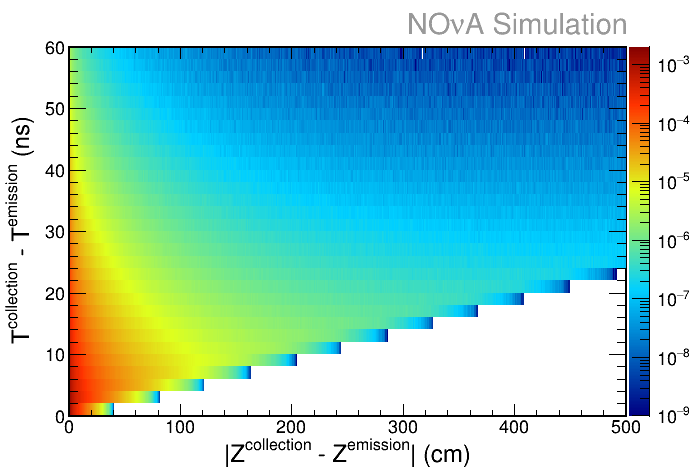
\includegraphics[width=.47\textwidth]{figures/SimPhotonCaputre.png} &
    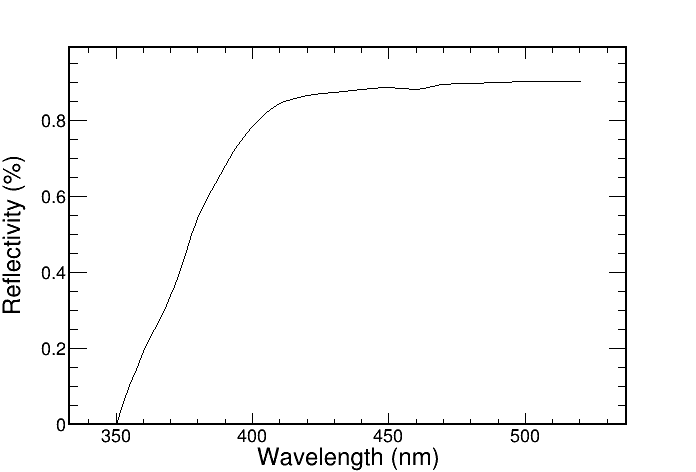
\includegraphics[width=.47\textwidth]{figures/SimWallReflectivity.png} \\
  \end{tabular}
  \caption[Simulation of Photon Transport]{Distributions used during the simulation of photon transport. Left: collection rate as a function of time and distance travelled from scintillator emission. Right: cell wall reflectivity as a function of wavelength.}
  \label{fig:SimPhoton}
\end{figure}

Next, the photons are transported through the fiber to the electronics. Since the fiber is looped and both ends are read out, half of the photons are transported to each end. The number of photons that reach the fiber ends is attenuated by applying an attenuation curve derived from quality control tests as a function of distance from the fiber end. Another template is constructed using a ray tracer that models transport time as a function of distance. The actual transport times are drawn from this template instead of handling the photon capture angles individually.

At this point in the simulation, there is a number of photons that reach the APD as a function of time. This is converted to photoelectrons (PEs) assuming a flat quantum efficiency of $0.85$ for every APD. The exact number of PEs collected is drawn from a log-normal distribution with a mean of the expected number of PEs to account for the repeated random charge avalanche process within the APD. The final output of the photon transport simulation is a set of objects that encodes the number of PEs as a function of time, called PhotonSignals.

\subsection{Electronic Readout}
\label{sec:Electronics}

The last piece of the detector simulation models the electronics readout. This section starts with the number of PEs collected by the APDs and simulates the effects of the electronics to generate the raw signals equivalent to data. Before the PE signal from the APD is input to the circuitry simulation, an excess noise factor is applied. The excess noise PE signal is drawn from a log-normal distribution, the limit of the product of many random variables, motivated by the fact that the actual PE signal comes from many random charge multiplications. Next, three chips on the FEBs are simulated, an application-specific integrated circuit (ASIC), an analong to digital converter (ADC), and a field-programmable gate array (FPGA).

The ASIC pre-amplifies and shapes the PE signal. A data driven effect is included at this point called APD sag, or the tendency when one APD channel observes a large hit for other channel baselines to slightly drop. The recovery from the drop can appear like real activity causing all APD pixels to register hits. Another form of noise is modeled at this point as the sum of two Gaussian Markov chains. This is done to simulate the high correlation of noise traces between adjacent samples, and is tuned to best match pedestal detector scans.

The shaped pulse is next input to the ADC, which performs two functions. The signal is first converted into an integer value, up to a maximum threshold that would saturate the ADC. These values are then sampled on a periodic basis to create a simulated time series of channel outputs. The FPGA then searches for peaks above threshold using a dual correlated sampling trace, defined from $ADC_i - ADC_{i - 3}$, where $ADC_j$ is the $j$th output from the ADC. A final type of noise is considered for otherwise empty cells, drawn probabilistically from templates made from histograms of ADC differences from data noise hits.

The hits above threshold are the final output of the detector simulation and are recorded as a vector of objects called RawDigits. This is the lowest level object that has the same format for both data and MC; however, the additional truth information is always stored for the MC for validation and further studies.

\subsection{Simulation Miscellany}
\label{sec:SimMisc}

In real data, readout did not always occur from every cell in the full detector. Full diblocks sometimes were missing due to original commissioning or repair work. Within individual diblocks, single channels can be masked off for too high noise levels or too low data rates. The diblock configuration for data was stored by run, and the channel masks were stored by subrun. To most accurately reflect the detector running conditions, the MC was generated matching the configurations in data, or weighting the MC configurations simulated by POT.

%\subsection{Oscillations and File Format}
%\label{sec:FluxSwap}

The FD MC files generated do not include any realistic oscillation probabilities; instead, three sets of files are produced. The first set assumes that there are no oscillations, called nonswap files. These files are consist of the same percentage of $\numu$ and $\nue$ generated naturally in the NuMI beam. The simulation does not generate any $\nutau$ so these events are entirely absent from nonswap files. The second set of files, called fluxswap, completely oscillate all $\numu$ to $\nue$, and vice versa. Finally, the third set of files, called tauswap, completely oscillate all $\numu$ and $\nue$ to $\nutau$. All three files include the same rate of NC events. Oscillation weights as a function of true energy can be applied individually to each interaction channel at a later stage, which allows for realistic conditions that can also be tuned without generating entirely new MC.

\section{Studying Simulation Files}

The benefits of retaining all of the information described in the previous sections is that it allows for quicker studies and validation. Truth information can be used to test the idealized proof of concept of a new analysis technique, and studies involving alternative flux models but no detector effects can be run without the time and computation expensive process of running the full simulation and reconstruction. Two packages were developed for these purposes, FluxReader and MCCheckOut.

FluxReader is a package designed to read and make distributions from Dk2Nu flux files \cite{ref:TNFR}. Like Dk2Nu files, FluxReader is experiment independent and can be used for any experiment that uses the NuMI beam line. Its main design is to create sets of spectra from the Dk2Nu files, where each spectrum in the set plots the same variable(s) but shows the distribution for a unique set of neutrino flavor, parent, applied cross section, and detector location. Users are able to configure nearly everything inside macros, thus eliminating the need for recompiling code.

FluxReader makes clever use of several existing capabilities within other packages to generate its sets of spectra. Every individual neutrino ray in the flux files is re-decayed to each detector configured in a particular FluxReader macro, so each flux file can populate spectra for both the \nova~ND and FD. The package is able to apply cross sections by reading in cross section splines from GENIE, since flux files by definition do not simulate detector interactions. The user is able to configure what cross sections are applied, with different spectra generated for each. In both of these cases, any additional histograms added to a particular set are handled automatically alleviating the need for user generated repetition of error prone code.

The strategy for evaluating beam related systematic errors was not to generate entirely new MC with systematically shifted quantities. Instead, only shifted Dk2Nu files were created, and ratios of shifted to nominal spectra as a function of true neutrino energy were generated for each neutrino flavor (also split by sign) and provided as event weights for the fully simulated MC. These studies were performed using the FluxReader framework \cite{ref:TNBeam}. The specific systematics are discussed in detail in chapter \ref{ch:Systs}.

While the systematic studies performed using FluxReader are the most directly related to the analysis in this dissertation, it has facilitated many other studies, from which a representative sample is briefly discussed below. The newest version of Fluka was compared against the previous version used in the \nova~simulation, a collaboration internal study necessary to help trace major simulation differences that might arise between major MC productions \cite{ref:FRFluka}. A proposal to run the NuMI beam with various different horn currents was supported with studies utilizing FluxReader \cite{ref:FRHornProposal}. This test was eventually carried out, and the FluxReader distributions were used for the MC predicted energy spectra compared to the data \cite{ref:FRHornResult}. Another study considered the effect of increasing the spacing between target fins to allow pions to more easily escape before scattering in a secondary target interaction \cite{ref:FRTarget}.

MCCheckOut is a package designed for validation of various sections of the \nova~simulation. It creates distributions of relevant variables for each step of the simulation to search for changes between different MC productions. Figure \ref{fig:MCCO_NDVtx} shown above is one of the standard plots created by MCCheckOut. Between major productions, modules are run that compare distributions for the MC truth, FLS hits, simulated POT, and RawDigits. MCCheckOut is typically run by a single person who pushes the results to an online webpage so that a wider audience can look for and comment on simulation differences. 

Ideally, only expected changes from simulation improvements are seen, but in reality, unexpected and unintended differences sometimes appear. It is vitally important to find and correct these mistakes before valuable computation time is wasted generating erroneous MC files. Several problems were discovered and fixed while this author was in charge of running simulation validation, two of which are briefly mentioned below. At one point, the window over which neutrino rays were sampled for FD interactions was shortened without taking into account the $3^\circ$ angle between the beam direction and detector. This led to an absence of events in a section of the detector, as shown in figure \ref{fig:MCCO_FD} \cite{ref:MCCO_FDFix}. A similar problem occurred later when a code change caused the location GENIE used to start to generating neutrino interactions at the ND to be pushed too far forward in Z. The result was an absence of events at the front of the detector, and specifically in the steel bookend, as shown in figure \ref{fig:MCCO_ND} \cite{ref:MCCO_NDFix}. MCCheckOut is clearly a valuable and necessary package for the MC simulation production.
\begin{figure}[htb]
  \centering
  \begin{tabular}{c c}
    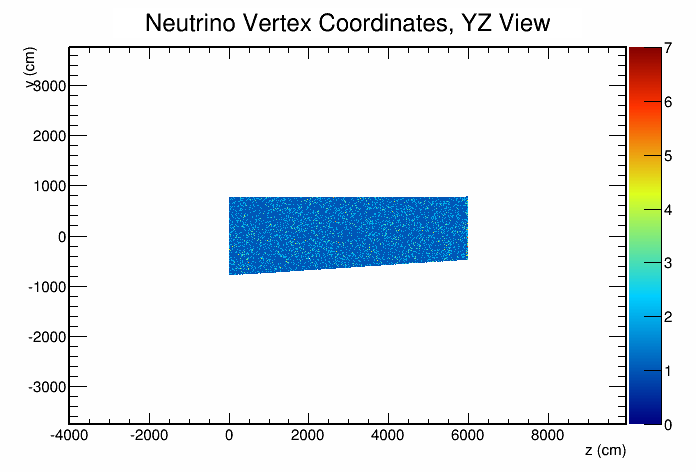
\includegraphics[width=.47\textwidth]{figures/MCCO_FDWrong.png} &
    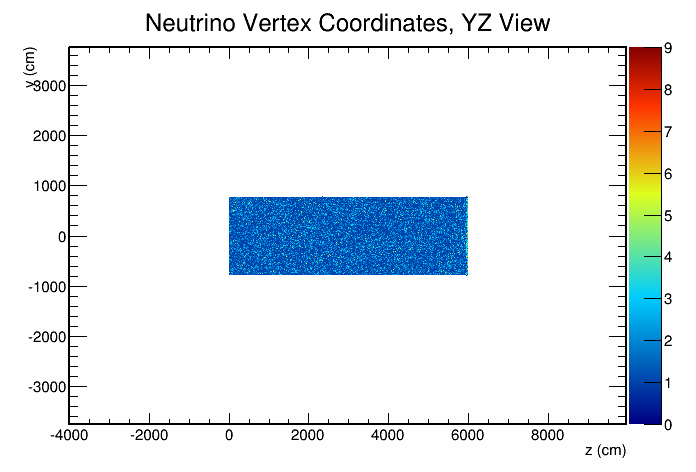
\includegraphics[width=.47\textwidth]{figures/MCCO_FDRight.png} \\
  \end{tabular}
  \caption[Identifying Missing Simulated Events in the FD]{Distribution of neutrino interaction vertices in the YZ view at the FD. The left plot shows a region of detector with no events due to a shortened flux window. The right plot shows the corrected distribution after the flux window was lengthened.}
  \label{fig:MCCO_FD}
\end{figure}

\begin{figure}[htb]
  \centering
  \begin{tabular}{c c}
    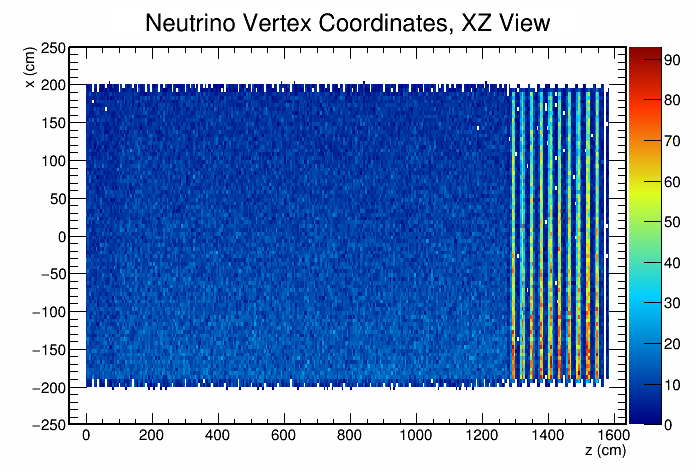
\includegraphics[width=.47\textwidth]{figures/MCCO_NDWrong.png} &
    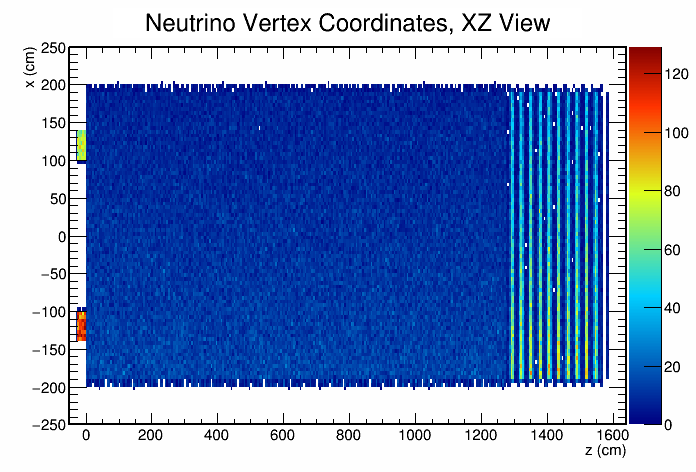
\includegraphics[width=.47\textwidth]{figures/MCCO_NDRight.png} \\
  \end{tabular}
  \caption[Identifying Missing Simulated Events in the ND]{Distribution of neutrino interaction vertices in the XZ view at the ND. Rock events were removed in these distributions. There are no interaction in the steel bookend in the left plot. On the right, the simulation was corrected and events can be seen within the bookend.}
  \label{fig:MCCO_ND}
\end{figure}